\documentclass{memo}
\usepackage{mathptm,mydef,myenv}
\usepackage{graphics,epsfig}
%\usepackage{MinionPro}
\usepackage[all]{xy}
\begin{document}
\small
\noindent{\large\bf{}C++ Object Model}


\paragraph{Simple object model}
In a simple object model, we maintain a table of slots, where each slot
contains a field (or pointer to a field) or a pointer to member function.

\paragraph{Two-table model for objects}
This is used in CORBA, SOM but not used in C++.
For this, we maintain two-slot structure for each object: one for \bb{fields}
and the other for \bb{methods}.

\paragraph{C++ object model}
Stroustrup's original C++ object model supports virtual functions in two
steps:
\bit
\w \bb{vtable (virtual table)}: a table of pointers to virtual functions is
  generated for each \bb{class}
\w \bb{vptr}: each object has a pointer, \bb+\_vptr+, which points to the
\bb{vtable}
\eit
\bb{vtpr} is set/reset/not-set through an instrumented code inserted to
\bb{constructors}, \bb{copy assignment operators\/}, etc.

\bb{vtable} contains a pointer to \bb{type\_info} objects for \bb{RTTI}
(runtime type identification). 


\paragraph{Virtual tables}
\bb{Virtual table} is a {\em lookup table of function pointers\/} used to
dynamically bind the virtual functions to objects at runtime. Every class that
uses virtual functions (or is derived from such a class) is given it's own
virtual table (\bb{vtable}) as a secret data member. 

The \bb{vtable} is setup
by the compiler at compile time. A virtual table contains \bb{one entry as a
function pointer for each virtual function} that can be called by objects of
the class.  Virtual table stores NULL pointer to pure virtual functions.

\paragraph{\_vptr}
The \bb{vtable pointer} or {\_vptr} is a hidden pointer added by the compiler
to the base class. And this pointer is pointing to the vtable of that
particular class. This \_vptr is inherited to all the derived classes. 

Each object of a class with virtual functions transparently stores this
\bb{\_vptr}. {\em Call to a virtual function by an object is resolved by following this
hidden \bb{\_vptr}\/}. 

\paragraph{Example: Code}
\begin{verbatim}
  class Base  
  {  
  public:  
    virtual void function1() {
      cout<<"Base :: function1()\n";
    };  
    virtual void function2() {
      cout<<"Base :: function2()\n";
    };  
    virtual ~Base(){};
  };  
   
  class D1: public Base  
  {  
  public:  
     ~D1(){};
     virtual void function1() { 
       cout<<"D1 :: function1()\n";
     };
  };  
  
  class D2: public Base  
  {  
  public:  
     ~D2(){};
     virtual void function2() { 
       cout<< "D2 :: function2\n";
     };  
  };  

  void main() {
    D1 *d = new D1;
    Base *b = d; 

    b->function1(); // prints "D1 :: function1()"
    b->function2(); // prints "Base :: function2()"
   
    delete b;
  }
\end{verbatim}

\begin{figure}
\begin{center}
\centerline{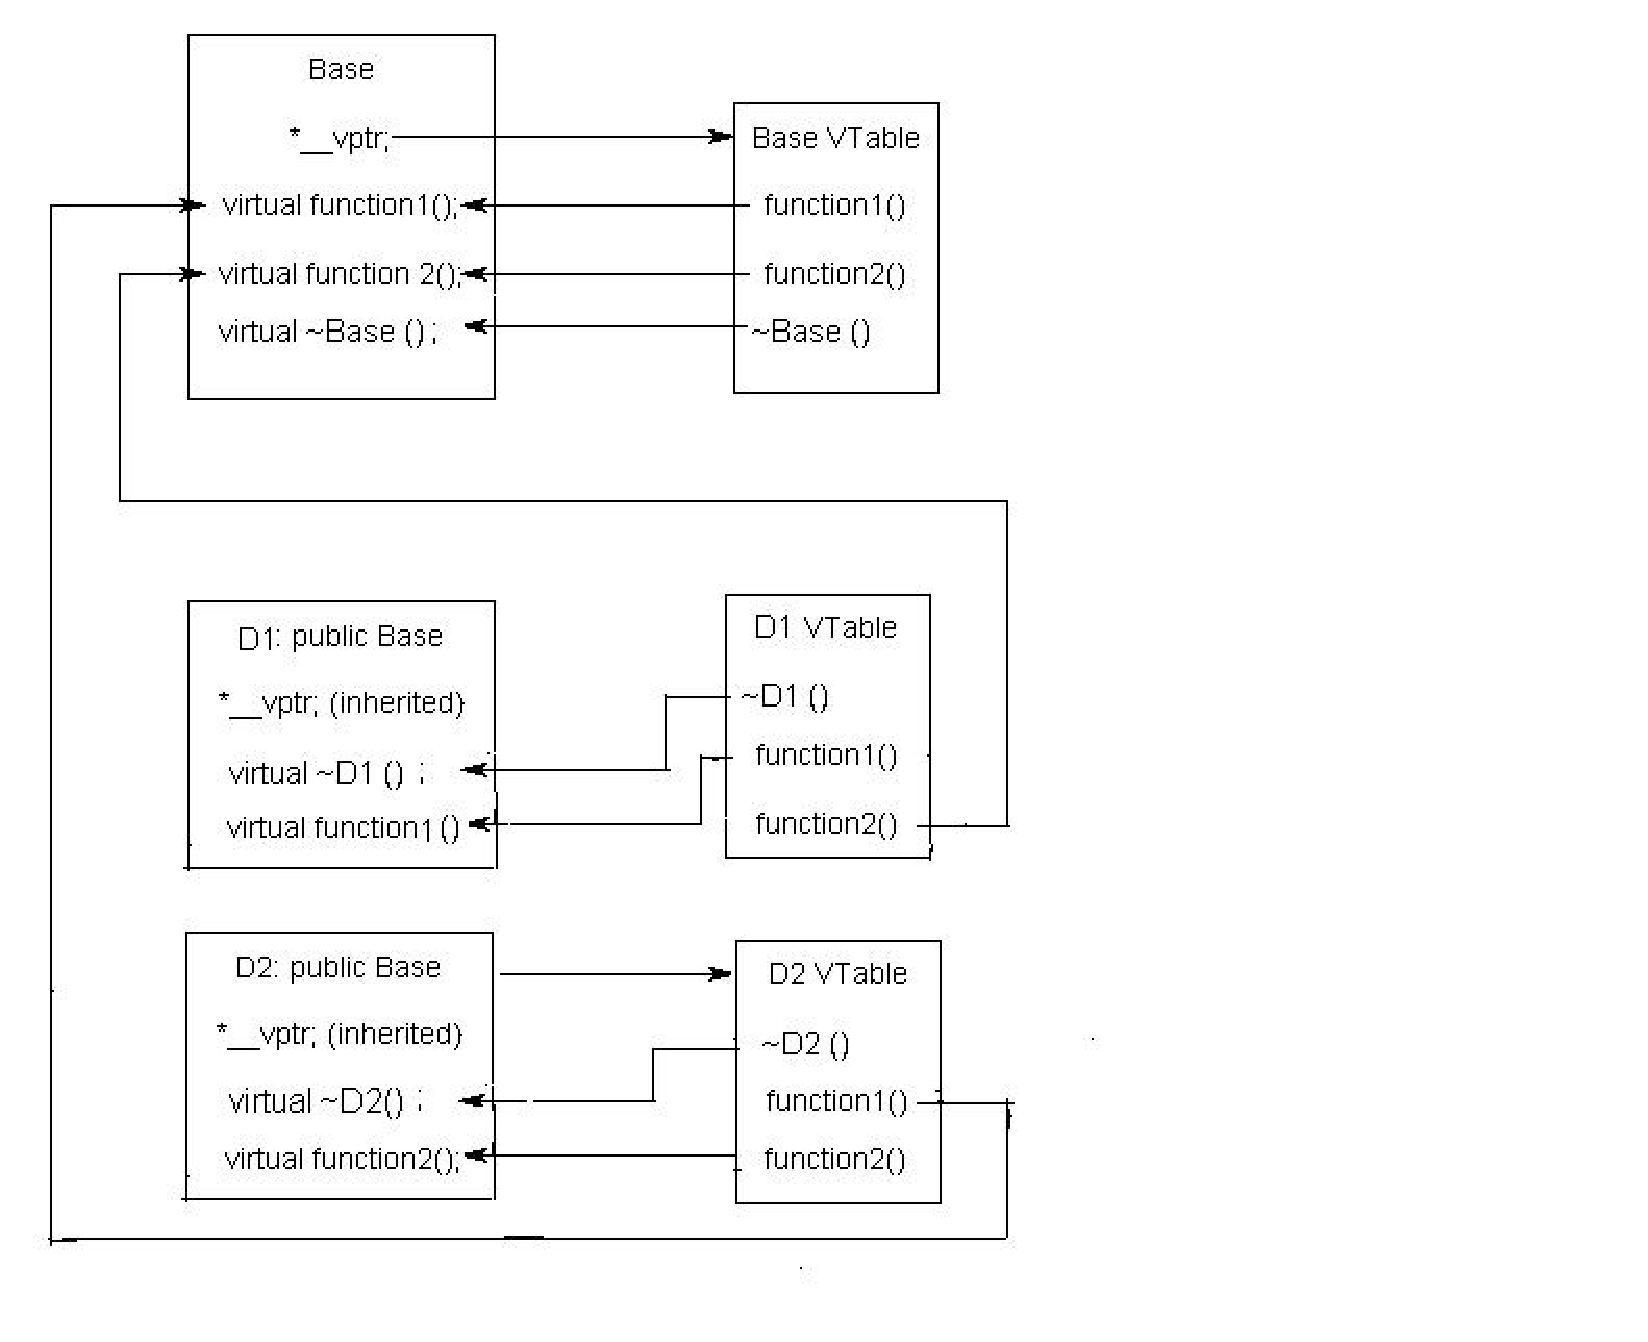
\epsfig{file=pics/vtable.eps,width=9cm}}
\end{center}
\caption{vtable, \_vptr for code example}
\end{figure}

In function \bb{main}, \bb{b} pointer gets assigned to \bb{D1's \_vptr} and
now starts pointing to \bb{D1's vtable}. Then calling to a function1(), makes
it's \_vptr calls D1's vtable function1() and so in turn calls D1's method
i.e. function1() as D1 has it's own function1() defined it's class. 

Where as pointer b calling to a function2(), makes it's \_vptr points to
\bb{D1's vtable} which in-turn pointing to Base class's vtable function2 () as
shown in the diagram (as D1 class does not have it's own definition or function2()). 

So, now calling delete on pointer \bb{b} follows the \_vptr -- which is
pointing to \bb{D1's vtable} calls it's own class's destructor i.e. D1 class's
destructor and then calls the destructor of Base class -- this as part of when
derived object gets deleted it turn deletes it's embedded base object. That's
why we must always make Base class's destructor as virtual if it has any
virtual functions in it. 


\paragraph{Instrumentation of virtual function calls}
\begin{verbatim}
  void main() {
    //D1 *d = new D1;
    d = _new(sizeof(D1));
    if (d != 0)
      px->D1::D1();

    //Base *b = d; // free

    //b->function1(); // prints "D1 :: function1()"
    (*b->_vtbl[2])(b);

    //b->function2(); // prints "Base :: function2()"
    (*b->_vtbl[3])(b);

    //delete b;
    if (b != 0) {
      (*b->_vtbl[1])(d); // destructor
      _delete(b);
    }
  }
\end{verbatim}

\end{document}

%%  LocalWords:  CORBA SOM lookup runtime vtable vptr destructor
